%%%%%%%%%%%%%%%%%%%%%%%% editor.tex %%%%%%%%%%%%%%%%%%%%%%%%%%%%%
%
% sample root file for the contributions of a "contributed volume"
%
% Use this file as a template for your own input.
%
%%%%%%%%%%%%%%%%%%%%%%%%%%%%% Springer %%%%%%%%%%%%%%%%%%%%%%%%%%


% RECOMMENDED %%%%%%%%%%%%%%%%%%%%%%%%%%%%%%%%%%%%%%%%%%%%%%%%%%%
\documentclass[graybox, envcountchap, natbib]{svmult}

% choose options for [] as required from the list
% in the Reference Guide

%\usepackage{type1cm}        % activate if the above 3 fonts are 
                             % not available on your system

\usepackage{makeidx}         % allows index generation
\usepackage{graphicx}        % standard LaTeX graphics tool
                             % when including figure files
\usepackage{multicol}        % used for the two-column index
\usepackage[bottom]{footmisc}% places footnotes at page bottom

\usepackage{newtxtext}       % 
\usepackage{newtxmath}       % selects Times Roman as basic font
\usepackage{doi}             % makes hyperlinks out of doi in bib

\usepackage{kantlipsum}
\usepackage{cleveref}

\let\Bbbk\relax              % MER: Fixes compilation error

% see the list of further useful packages in the Reference Guide
\usepackage{chapterbib}
\usepackage{etoolbox}
\usepackage{url}
\usepackage{tikz}
\usepackage{parskip}
\usepackage{multicol}
\usepackage{multirow}
\usepackage{makecell}
\usepackage{subcaption}
\usepackage{verbatim}
\usepackage{comment}
\usepackage{adjustbox}
\usepackage{lastpage}
\usepackage{bm}
\usepackage{textcomp}
\usepackage{array}
\usepackage{amsmath}
\usepackage{amsfonts}
%\usepackage{amssymb}
\usepackage{mathtools}
\usepackage[ruled]{algorithm2e}
\usepackage{hyperref}
\usepackage{booktabs} % MER: Prettier tables
\usepackage{siunitx} % JR: easy SI-adhering quantities


\usepackage{xcolor}
\usepackage{listings}
\usepackage[most]{tcolorbox} 	%used for writing process notes, code boxes 
\usepackage{fancybox}
\usepackage{fancyvrb}		    %provides tab and white space preservation for 
%the verbatim environment. Needed for Python

% added for code snippets:
\usepackage{pythonhighlight}
\usepackage{todonotes}
\usepackage{lipsum}
\usepackage{fancybox}

\newcommand{\Cass}{\mathrm{Ca}_{\mathrm{ss}}}
\newcommand{\Cai}{\mathrm{Ca}_{\mathrm{i}}}
\newcommand{\Ca}{Ca$^{2+}$\;}
%\newcommand{\dt}{\Delta t}

% \allowdisplaybreaks


\newcommand{\dokken}[1]{\todo[inline,color=red!50, caption={2do}]{
    \begin{minipage}{\textwidth-4pt}
      \underline{Dokken:} #1
    \end{minipage}}}

\newcommand{\A}[1]{{\textcolor{red}{#1}}}        %Aslak
\definecolor{mollygreen}{rgb}{0.0,0.5,0.0}
\definecolor{mollyred}{rgb}{0.5,0,0}
\newcommand{\M}[1]{{\textcolor{mollygreen}{#1}}}        %Molly 
\newcommand{\Mred}[1]{{\textcolor{mollyred}{#1}}} %Mollyquestion

\makeatletter
\renewcommand{\algocf@makecaption}[2]{% no singleline check
  \parbox[t]{\columnwidth}{\algocf@captiontext{#1}{#2}}%
}%
\renewcommand{\algocf@makecaption@boxed}[2]{%
  \global\sbox\algocf@capbox{\algocf@makecaption{#1}{#2}}%
}%
\renewcommand{\algocf@caption@boxed}{\vskip\AlCapSkip
  \leavevmode\hskip-\leftskip\box\algocf@capbox\hskip-\rightskip}
\makeatother


\newcommand{\emp}[1]{\texttt{#1}}

\newcommand{\button}[1]{\ovalbox{{#1}}}


%\newenvironment{programcode2}[1]{\newline \ignorespaces\def\stmtopen##1{##1}%{\small{#1}}}%

\newenvironment{programcode2}[1]{\ignorespaces\def\stmtopen##1{##1}{\vspace*{0.5cm}\par \small{#1}}}{\noindent\textcolor{programcode}{\rule{\columnwidth}{0pt}}\par\addvspace{\baselineskip}}%



\newcommand{\ubuntu}[1]{
  \vspace{-1em}
  \begin{programcode}{}
    \colorbox{blue!10}{\parbox{0.98\textwidth}{\textcolor{black}{\texttt{#1 \hfill (Ubuntu)}}}}
  \end{programcode}
  \vspace{-0.5em}
}

\definecolor{deepblue}{rgb}{0,0,0.5}
\definecolor{deepred}{rgb}{0.6,0,0}
\definecolor{deepgreen}{rgb}{0,0.5,0}
\definecolor{codebox}{gray}{0.92}
\usepackage{accsupp}

\lstdefinestyle{BashStyle}{
  language=bash,
  basicstyle=\ttfamily,
  otherkeywords={self},
  keywordstyle=\color{deepblue},
  emphstyle=\ttb\color{deepred},
  stringstyle=\color{deepgreen},
  commentstyle=\color{blue},
  frame=tb,
  showstringspaces=false,
  backgroundcolor = \color{codebox},
  breaklines=true,
  columns=fullflexible,
  breakatwhitespace=true,
  prebreak=\textbackslash,
  postbreak=\raisebox{0ex}[0ex][0ex]{\BeginAccSupp{ActualText={}}\ensuremath{\color{red}\hookrightarrow}\EndAccSupp{}}
}

% Custom terminal environment which puts dollars in front of commands
\newcommand\dollarasnumber[1]{\ttfamily\$}
\lstdefinestyle{TerminalStyle}{
  xleftmargin=2.0em,
  framexleftmargin=2.0em,
  language=bash,
  basicstyle=\ttfamily,
  otherkeywords={self},
  keywordstyle=\color{deepblue},
  emphstyle=\ttb\color{deepred},
  stringstyle=\color{deepgreen},
  commentstyle=\color{blue},
  showstringspaces=false,
  backgroundcolor = \color{blue!10},
  breaklines=true,
  columns=fullflexible,
  breakatwhitespace=true,
  prebreak=\textbackslash,
  numbers=left,
  numberstyle=\dollarasnumber,
  %postbreak=\raisebox{0ex}[0ex][0ex]{\BeginAccSupp{ActualText={}}\ensuremath{\color{red}\hookrightarrow}\EndAccSupp{}}
}


\def\fenics{FEniCS}
\def\svmtk{SVM-Tk}
\def\svmtkfull{Surface-Volume-Meshing Toolkit}
\def\btk{BrainToolKit}
\def\freesurfer{FreeSurfer }
\def\paraview{ParaView}
\def\ftetwild{fTetWild}
\def\pyvista{PyVista}
\def\kdfull{K$3$D Jupyter}
\def\k3d{K$3$D}
\def\multiphenics{Multiphenics}
\def\freeview{Freeview}
%--------------------------------
%  Collaboration 
%--------------------------------
\newcommand{\citeme}{\textcolor{red}{(Reference needed)}}
\newcommand{\fixme}[1]{\textcolor{red}{#1}}

\newcommand{\kam}[1]{\todo[inline,color=green!10]{KAM: #1}}
\newcommand{\kent}[1]{\kam{#1}}
\newcommand{\lmv}[1]{\todo[inline,color=green!20]{LMV: #1}}
\newcommand{\mer}[1]{\textcolor{magenta}{#1}}

% ----------------------- %
% ---- Theorems, etc ---- %
% ----------------------- %

\newtheorem{thm}{Theorem}[section]
\newtheorem{cor}[thm]{Corollary}
\newtheorem{lem}[thm]{Lemma}
\newtheorem{prop}[thm]{Proposition}
\newtheorem{exmp}[thm]{Example}

%%
% equation counter will be reset at the start of each section
\numberwithin{equation}{chapter}

% ------------------------------ %
% ---- Math definitions -------- %
% ------------------------------ %
%matrices
\newcommand{\R}{\mathbb{R}}

\newcommand{\Id}{\mathbb{I}}

%\newcommand{\vecnot}[1]{\mathbf{#1}}
\newcommand{\vecnot}[1]{#1}
\newcommand{\vu}{\vecnot{u}}
\newcommand{\vf}{\vecnot{f}}
\newcommand{\vg}{\vecnot{g}}
\newcommand{\vn}{\vecnot{n}}
%\newcommand{\vv}{\vecnot{v}}
\newcommand{\vx}{\vecnot{x}}
\newcommand{\vp}{\vecnot{p}}
\newcommand{\vq}{\vecnot{q}}
\newcommand{\vG}{\vecnot{G}}

% mathematical operators
\DeclareMathOperator*{\esssup}{ess\,sup}
\DeclareMathOperator{\Div}{\mathrm{div}}
\DeclareMathOperator{\Curl}{\mathrm{curl}}
\DeclareMathOperator{\Grad}{\nabla}
\DeclareMathOperator{\trace}{\mathrm{tr}}

\newcommand{\suml}[2]{\ensuremath{\sum\limits_{#1}^{#2}}}
\newcommand{\tr}[1]{\trace\left(#1\right)}
\newcommand{\sig}[1]{\sigma\left(#1\right)}
\newcommand{\e}[1]{\varepsilon\left(#1\right)}

% inner products / duality pairings 
\newcommand{\inner}[2]{\langle #1,#2\rangle}
\newcommand{\innerwtd}[3]{\inner{#1}{#2}_{#3}}

% norms
\newcommand{\nrmbar}[1]{\vert\vert #1 \vert\vert}
\newcommand{\nrm}[2]{\nrmbar{#1}_{#2}}

% inequalities 
\newcommand{\ls}{\lesssim} %needs \usepackage{amsmath,amssymb}

% tensor notation
\newcommand{\tnsr}[1]{#1}


% ------------------------------------------------------
% Used to create a consistent command line command
% appearance for tutorials
% ------------------------------------------------------ 
\newcommand{\hedr}[1]{\noindent {\large \textbf{#1}}\\}

% Paths used in the text
\newcommand\dirstyle[1]{\texttt{#1}} %% MER says: Use this one
\def\coderoot{src/mri}
\def\abbydicom{dicom/abby}
\def\erniedicom{dicom/ernie} % Raw MRI data from ernie
\def\ernieT1{dicom/ernie/T13D} % Extracted MRI series from dicom/ernie
\def\ernieoutput{freesurfer/ernie} % Output from freesurfer
\def\fenicsdiffusion{fenics/diffusion} % Output from freesurfer

\def\mridataroot{\emp{FIXME}}
\def\mridataseq{\emp{FIXME-T13D}}


\def\mriTONEdataseq{\emp{MRI-Series-T13D}}
\def\mriTTWOdataseq{\emp{MRI-Series-T23D}}
\def\mriDTIdataseq{\emp{MRI-Series-DTI3D}}


%\def\freesurfer{\dirstyle{freesurfer}}

% the `command prompt' formatting utility
\def\dir[#1]{{\textasciitilde}/#1}
%usage: \cmdprmpt{current directory}{command}
\newcommand{\cmdprmpt}[2]{\text{dir[#1]\$} #2}

% Simple command prompt
\newcommand{\smpprmpt}[1]{\text{\$ }#1}
\newcommand{\outprmpt}[1]{#1}
% text symbols
\def\dash{\texttt{-}}
\def\ddash{\texttt{-{}-}}

% misc text names
\def\subjid{ernie}
\def\fenics{FEniCS}
%\def\svmtk{SVM-Tk}
\def\svmtkfull{Surface-Volume-Meshing Toolkit}
\def\btk{BrainToolKit}
%\def\freesurfer{FreeSurfer}

% Others macros
\newcommand{\mesh}{\mathcal{T}}
\newcommand{\dx}{\, \mathrm{d}x}
\newcommand{\dt}{\, \mathrm{d}t}

% Used for image placement
\def\imagetop#1{\vtop{\null\hbox{#1}}}

\definecolor{codebox}{gray}{0.92}
\definecolor{amber}{rgb}{1.0, 0.75, 0.0}
\definecolor{bananamania}{rgb}{0.98, 0.91, 0.71}
\definecolor{goldenpoppy}{rgb}{0.99, 0.76, 0.0}


\newcommand{\freesurfernote}[1]{
  \begin{tcolorbox}[width=\textwidth ,colback=bananamania!50,title={\textbf{Freesurfer comments}},colbacktitle=bananamania!20,coltitle=black,arc =0pt,colframe=black,lefttitle=0.35\textwidth ,
      outer arc = 0pt,
      titlerule = 0pt]
    #1
  \end{tcolorbox}
}


\newcommand{\name}[1]{"#1"}


% ------------------------------ %
%      python code style         %
% ------------------------------ %
% Default fixed font does not support bold face
\DeclareFixedFont{\ttb}{T1}{txtt}{bx}{n}{10} % for bold
\DeclareFixedFont{\ttm}{T1}{txtt}{m}{n}{10}  % for normal

% Custom colors
\definecolor{deepblue}{rgb}{0,0,0.5}
\definecolor{deepred}{rgb}{0.6,0,0}
\definecolor{deepgreen}{rgb}{0,0.5,0}
\definecolor{codebox}{gray}{0.92}


% MER: These Python commands depend on \usepackage{pythonhighlight}


% Python for inline
\newcommand\pythoninline[1]{\pyth{#1}}

\newcommand{\terminaltilde}{\raisebox{-0.5ex}{\textasciitilde}}

%% \newcommand{\lstvdots}{%
%%   \vbox{\baselineskip3pt\lineskiplimit0pt\kern1pt\hbox{.}\hbox{.}\hbox{.}\kern-1pt}}
\def\CC{{C\nolinebreak[4]\hspace{-.05em}\raisebox{.4ex}{\tiny\bf ++}}}

\newcommand\namestyle[1]{\emp{#1}}

% Make breakline arrow non-selectable

\lstdefinestyle{CStyle}{
  language=c++,
  basicstyle=\ttfamily ,
  keywordstyle=\ttb\color{deepblue},
  emph={class},
  emphstyle=\ttb\color{deepred},
  stringstyle=\color{deepgreen},
  commentstyle=\color{blue},
  columns=fullflexible,
  frame=single,
  showstringspaces=false,
  backgroundcolor = \color{codebox},
  breaklines=true,
  postbreak=\raisebox{0ex}[0ex][0ex]{\BeginAccSupp{ActualText={}}\ensuremath{\color{gray}\hookrightarrow}\EndAccSupp{}}
}


\makeindex             % used for the subject index
                       % please use the style svind.ist with
                       % your makeindex program

%%%%%%%%%%%%%%%%%%%%%%%%%%%%%%%%%%%%%%%%%%%%%%%%%%%%%%%%%%%%%%%%%

\begin{document}

\frontmatter%%%%%%%%%%%%%%%%%%%%%%%%%%%%%%%%%%%%%%%%%%%%%%%%%%%%%%

%%%%%%%%%%%%%%%%%%%%%%% dedic.tex %%%%%%%%%%%%%%%%%%%%%%%%%%
%
% sample dedication
%
% Use this file as a template for your own input.
%
%%%%%%%%%%%%%%%%%%%%%%%% Springer Nature%%%%%%%%%%%%%%%%%%%%%%%%%%

\begin{dedication}
A Rosy e Wolmer
\end{dedication}




%%%%%%%%%%%%%%%%%%%%%%foreword.tex%%%%%%%%%%%%%%%%%%%%%%%%%%%
% sample foreword
%
% Use this file as a template for your own input.
%
%%%%%%%%%%%%%%%%%%%%%%%% Springer %%%%%%%%%%%%%%%%%%%%%%%%%%

\foreword

%% Use the template \textit{foreword.tex} together with the document class SVMono (monograph-type books) or SVMult (edited books) to style your foreword\index{foreword}. 

%% The foreword covers introductory remarks preceding the text of a book that are written by a \textit{person other than the author or editor} of the book. If applicable, the foreword precedes the preface which is written by the author or editor of the book.


\vspace{\baselineskip}
\begin{flushright}\noindent
Place\hfill {\it Foreword author}\\
\end{flushright}


%%%%%%%%%%%%%%%%%%%%%%preface.tex%%%%%%%%%%%%%%%%%%%%%%%%%%%%%%%%%%%%%%%%%
% sample preface
%
% Use this file as a template for your own input.
%
%%%%%%%%%%%%%%%%%%%%%%%% Springer %%%%%%%%%%%%%%%%%%%%%%%%%%

% NON PENSO MI SERVA
% \preface

%\vspace{\baselineskip}
%\begin{flushright}\noindent
%Place, Date
%\hfill{\it Editors}\\
%\end{flushright}

%%%%%%%%%%%%%%%%%%%%%%acknow.tex%%%%%%%%%%%%%%%%%%%%%%%%%%%%%%%%%%%%%%%%%
% sample acknowledgement chapter
%
% Use this file as a template for your own input.
%
%%%%%%%%%%%%%%%%%%%%%%%% Springer %%%%%%%%%%%%%%%%%%%%%%%%%%

\extrachap{Acknowledgements}

%I would like to express my heartfelt gratitude to my PhD advisor, Dr. Riccardo Munaf\'o, and my supervisor, Prof. Emiliano Votta, for their guidance and unwavering support throughout this journey.

% @@@ Non credo sia questo il tipo di ringraziamento che intendono le guidelines, tanto più che sono ringraziamenti a nome di tutti gli autori, quindi sarebbe strano avere degli autori che si autoringraziano. Negli Acknowledgements di solito si citano eventuali fonti di finanziamento, oppure persone/istituzioni che non compaiono tra gli autori ma hanno permesso di sviluppare il lavoro fornendo qualche forma di aiuto esterno (ad esempio fornendo dati o consigli). 



\setcounter{tocdepth}{0}
\tableofcontents
%%%%%%%%%%%%%%%%%%%%clist.tex %%%%%%%%%%%%%%%%%%%%%%%%
%                                                    
% sample list of contributors and their addresses    
%                                                    
% Use this file as a template for your own input.    
%                                                    
%%%%%%%%%%%%%%%%%%%%%%%% Springer %%%%%%%%%%%%%%%%%%%%
\contributors

\begin{thecontriblist}
Sara Paratico$^1$

Riccardo Munaf\'o$^1$

Chiara Trenti$^{2,3}$

Petter Dyverfeldt$^{2,3}$

Simone Saitta$^4$

Emiliano Votta$^1$

\vspace{1cm}

$^1$ Politecnico di Milano, Department of Electronics, Information, and Bioengineering, Milano, Italy

$^2$  Division of Cardiovascular Medicine, Department of Health, Medicine and Caring Sciences, Link\"oping University, Universitetssjukhuset, 581 83 Linköping, Sweden

$^3$  Center for Medical Image Science and Visualization (CMIV), Link\"oping University, 
Universitetssjukhuset, 581 83 Linköping, Sweden

$^4$ Amsterdam University Medical Center, 
Department of Biomedical Engineering and Physics, Amsterdam, The Netherlands

\end{thecontriblist}

%%%%%%%%%%%%%%%%%%%%%%acronym.tex%%%%%%%%%%%%%%%%%%%%%%%%%%%%%%%%%%%%%%%%%
% sample list of acronyms
%
% Use this file as a template for your own input.
%
%%%%%%%%%%%%%%%%%%%%%%%% Springer Nature%%%%%%%%%%%%%%%%%%%%%%%%%%

\extrachap{Acronyms}

Use the template \emph{acronym.tex} together with the document class SVMono (monograph-type books) or SVMult (edited books) to style your list(s) of abbreviations or symbols.

Lists of abbreviations\index{acronyms, list of}, symbols\index{symbols, list of} and the like are easily formatted with the help of the Springer Nature enhanced \verb|description| environment.

\begin{description}[CABR]
\item[ABC]{Spelled-out abbreviation and definition}
\item[BABI]{Spelled-out abbreviation and definition}
\item[CABR]{Spelled-out abbreviation and definition}
\end{description}

\mainmatter%%%%%%%%%%%%%%%%%%%%%%%%%%%%%%%%%%%%%%%%%%%%%%%%%%%%%%%

% %%%%%%%%%%%%%%%%%%%%%part.tex%%%%%%%%%%%%%%%%%%%%%%%%%%%%%%%%%%
% 
% sample part title
%
% Use this file as a template for your own input.
%
%%%%%%%%%%%%%%%%%%%%%%%% Springer %%%%%%%%%%%%%%%%%%%%%%%%%%

\begin{partbacktext}
\part{Part Title}
\noindent Use the template \emph{part.tex} together with the document class SVMono (monograph-type books) or SVMult (edited books) to style your part title page and, if desired, a short introductory text (maximum one page) on its verso page.

\end{partbacktext}
% Write the full path to the location of the graphics relative to book.tex
\graphicspath{{chapters/chp1/graphics/}}

\title{Estimation of optimal inlet boundary conditions for blood flow assessment in abdominal aortic aneurysm using variational data assimilation}
\titlerunning{Paratico et al.}

\author{S.~Paratico, R.~Munaf\`o, C.~Trenti, P.~ Dyverfeldt, S. Saitta and E.~Votta}
\authorrunning{Paratico et al.}

\institute{S.~Paratico \email{sara.paratico@mail.polimi.it} \at Politecnico di Milano}
% @@@ fossi in te, fornirei l'indirizzo email del Politecnico: è più istituzionale e l'inzirizzo con dominio mail.polimi.it resta attivo a vita. --> ## FATTO !
\maketitle

\abstract{}
%Abdominal aortic aneurysms (AAAs) are a life-threatening cardiovascular condition characterized by a permanent dilation of the abdominal aorta. Diagnosis before rupture is critical due to its often asymptomatic nature. Hemodynamic assessment through numerical simulations or 4DFlow magnetic resonance imaging (MRI) can help diagnosis and risk stratification of AAAs. However, each method has limitations: computational fluid dynamics (CFD) relies on assumptions and model constraints, while 4DFlow MRI suffers from low resolution and it is affected by noise. Data assimilation (DA) integrates numerical models with 4D flow MRI to enhance resolution and reduce noise, offering a promising solution. This study focuses on optimizing inlet boundary conditions (BCs) using variational data assimilation (VarDA), aiming to minimize discrepancies between a CFD solution obtained with an incremental pressure correction scheme (IPCS), and in vivo velocity measurements from 4DFlow MRI in AAAs. The goal of this study was to develop and evaluate a computationally efficient DA approach for accurate non-invasive reconstruction of AAA blood flow dynamics. 

Blood fluid dynamics impacts vessel wall cells and tissue biomechanics, influencing thrombus formation and vessel wall remodeling. Accurate \textit{in vivo} quantification can thus aid in understanding these mechanisms and patient stratification. Computational fluid dynamics (CFD) and 4D flow MRI are used for this purpose, but both have limitations: CFD involves assumptions and boundary condition simplifications, while 4D flow MRI suffers from low spatial resolution and noise. This study employs variational data assimilation (VarDA) to integrate CFD and 4D flow MRI, yielding a high-resolution, noise-free flow field closely aligned with 4D flow MRI velocity data. To enhance alignment, the optimal inlet velocity profile is determined iteratively via an incremental pressure correction scheme (IPCS). Previously tested in simple synthetic geometries and later in a complex patient-specific abdominal aortic aneurysm (AAA), this approach demonstrates improved reliability in patient-specific hemodynamic evaluation.
% @@@ Espanderei l'ultima frase per i) accennare anche ai benchmark sintetici e ii) dare almeno un paio di risultati esemplificativi delle prestazioni del metodo. Attualmente l'abstract è di 178 parole; di solito gli abstract ne prevedono al massimo 250, quindi possiamo aggiungere fino a 72 parole, che non sono affatto poche.  


\section*{Introduction}
%AAAs are characterized by localized aortic dilations, altering hemodynamics and increasing rupture risk [\cite{Lattanzi2020}]. Assessing this risk is complex, relying on morphology, patient-specific factors like age, medical history and aneurysm progression. Fluid-dynamic parameters show promise as rupture predictors [\cite{Bologna2023}] and can be quantified through the analysis of clinical imaging, namely of 4DFlow MRI [\cite{Dyverfeldt2015}], or through patient-specific CFD models [\cite{Salman2021}]. However, the former approach provides indirect measurements of blood velocity, which are noisy, to the point they typically violate the mass conservation law, and are characterized by low spatiotemporal resolution. On the other hand, CFD models compute a noiseless and extremely well resolved blood velocity field, but the latter heavily depends on BCs that are typically unknown, and hence set based on simplifying assumptions or affected by uncertainty. VarDA offers a rigorous framework to merge the two approaches, reduce the impact of the respective limitations while leveraging the respective potential. By incorporating velocity observations obtained through 4D flow MRI within CFD simulations of blood flow, VarDA computes noiseless and highly resolved velocity data that by construction respect the conservation of mass while enforcing their consistency with experimental observations that are not based on simplifying assumptions. However, studies based on VarDA have also highlighted that its application to 3D problems in geometrically complex domains is far from trivial and can be hampered by high computational costs. 

Alterations in blood fluid dynamics often contribute to the onset or the progress of cardiovascular pathological conditions [\cite{Bappoo2021}, \cite{Guzzardi2015}]. Hence, quantifying blood fluid dynamics on a patient-specific basis and non-invasively can support the understanding of pathological mechanisms or the stratification of patients based on the risk for adverse endpoints. To this aim, blood flow field can be reconstructed from clinical imaging, namely 4D flow MRI [\cite{Dyverfeldt2015}], or computed through patient-specific CFD models  [\cite{Kheyfets2015}]. 
However, 4D flow MRI provides indirect and noisy velocity measurements with low spatio-temporal resolution, which often violate mass conservation. On the other hand, CFD models, which solve the discretized version of the Navier-Stokes (NS) equations to compute noise-free and well-resolved velocity fields, are not immune to numerical artefacts %such as dispersion or diffusion and may not always achieve the desired resolution. Moreover, CFD simulations 
and typically rely on simplifying assumptions for boundary conditions (BCs), including inlet velocity BCs. 
Variational data assimilation (VarDA) combines physical governing equations with sparse, uncertain experimental data by optimizing initial or boundary conditions to minimize the misfit between simulation results and data. In cardiovascular fluid dynamics, VarDA merges CFD-based Navier-Stokes equations with in vivo 4D flow MRI velocity data, minimizing the misfit by optimizing the inlet velocity profile. A challenge is computing both the velocity and pressure gradient fields, particularly in large arteries with high velocities, requiring pressure-velocity coupling or correction schemes. However, noise in the velocity field, particularly from MRI data, can hinder proper pressure field correction in these schemes.

\subsection*{Related works}
\label{sec:background}

Several studies have explored VarDA in hemodynamics, ranging from 2D steady-state conditions to 3D transient conditions.
\cite{Delia2012} showed that 
VarDA allows to reconstruct flow fields in geometrically complex 2D domains, such as the 2D representation of the aortic arch and carotid bifurcation, even with noisy velocity data. Subsequently, in \cite{Delia2013}, they same authors showed that, in 2D domains, noisy velocity data can be effectively managed by properly managing inlet BCs. In particular, they showed that the regularization of the inlet velocity profile through the use of a control variable also regularized the velocity field over the whole domain and allowed for successful pressure-velocity coupling.
\cite{Tiago2017} extended VarDA to a 3D saccular aneurysm, demonstrating its flexibility with various BCs and optimization methods like gradient-based and genetic algorithms to improve accuracy. \cite{Koltukluoglu2018} showed that VarDA, applied to 4D Flow MRI data, outperformed traditional CFD methods by dynamically adjusting boundary conditions in real-time to maintain flow congruence near inlets. \cite{Funke2019} demonstrated the effectiveness of 4D (3D space + time) VarDA in capturing transient blood flow in aneurysms using phase contrast-MRI data. Finally, \cite{Dokken2020} proposed a multimesh finite element (FE) method that enhanced stability and accuracy by allowing flexible BC management across multiple mesh domains, which is key for simulating complex hemodynamics in realistic geometries.

\subsection*{Aim of the work}
This study aims to implementing a method to compute \textit{in vivo} blood fluid dynamics on a patient-specific basis with high space-resolution without using simplifying hypotheses on the inlet BCs. To this aim, we leverage VarDA to estimate an optimal inlet BC for a CFD simulation, where the inlet BC initially consists in a noisy and uncertain 4D flow MRI-based velocity profile, and consistency between the CFD-computed velocity field and sparse 4D flow MRI-based data in the bulk flow region is enforced. 
We benchmarked the method on ideal 2D and 3D geometries and then applied it to a patient-specific abdominal aortic aneurysm (AAA) geometry. 

\section*{Methods}
\label{sec:methods}

\subsection*{Data Assimilation Method}
The VarDA approach was formulated as an optimization problem constrained by the NS equations, using the \emph{dolfin-adjoint} library for the adjoint problem. The process follows three steps: running a first numerical simulation with tentative inlet BCs (which we refer to as the \emph{forward model} or \emph{Tape}), solving the optimization problem to identify inlet BCs, and running a final numerical simulation yielding the refined velocity and pressure fields (Fig. \ref{fig:scheme}).

\begin{figure}
    \centering
    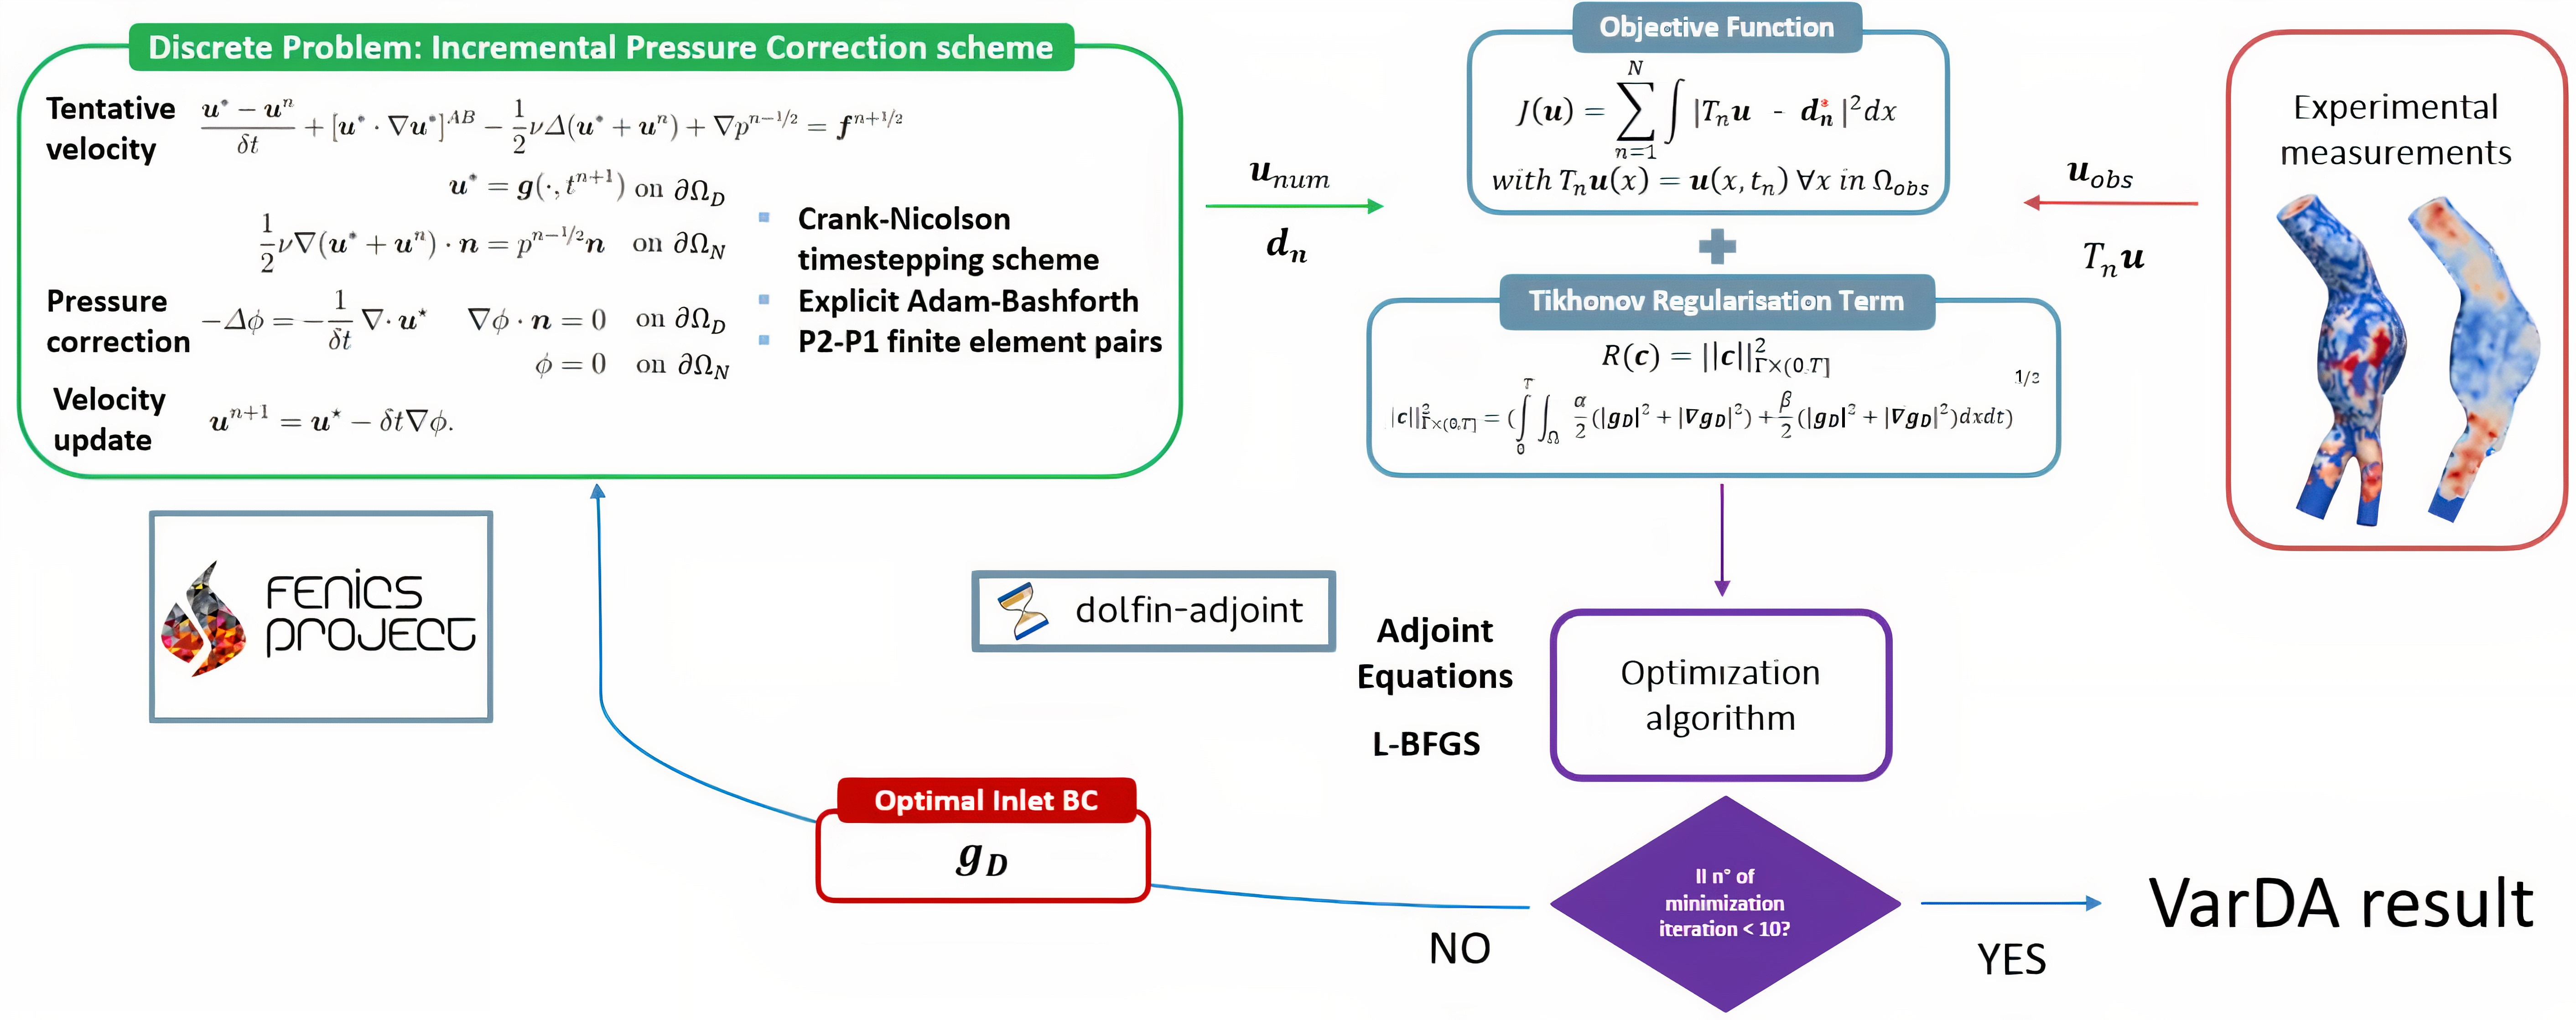
\includegraphics[width=\textwidth]{chapters/chp1/graphics/schema2_upscaled4.jpg}
    \caption{\small \textbf{Top-left}: The finite element (FE) solver computes the Navier-Stokes (NS) equations with an initial guess for the inlet boundary conditions (BCs); \textbf{Top-right}: experimental velocity measurements are taken at discrete points in the domain; \textbf{Center}: discrepancy between the computational fluid dynamics (CFD) velocity field and experimental data is minimized by iteratively refining inlet velocity profile with a gradient-based method.}
    \label{fig:scheme}
\end{figure}

%\subsection*{Governing equations of the problem}
%Blood fluid dynamics follows the NS equations, which express the conservation of linear momentum and mass. Modeling blood as a Newtonian, incompressible fluid [\cite{Stokes2009}], the Eulerian form of the momentum equations reads:

%\begin{equation}
%\label{eq:1}
%\small
%\rho_f \left( \frac{\partial \mathbf{u}}{\partial t} + (\mathbf{u} \cdot \nabla \mathbf{u}) \right) - \nabla \cdot \mathbf{T}_f(\mathbf{u}, p) = \rho_f \mathbf{f} \quad \forall x \in \Omega, \quad t > 0
%\end{equation}

%where \(\mathbf{f} = \mathbf{f}(\mathbf{x},t)\) represents volumetric forces, \(\rho_f\) is blood density ($1.06 \, g/cm^3$ [\cite{Timothy2016}]), and \(\mathbf{T}_f(\mathbf{u}, p)\) is the Cauchy stress tensor defined as:


%\begin{equation}
%\label{eq:2}
%\small
%\mathbf{T}_f(\mathbf{u}, p) = -p\mathbf{I} + \mu(\nabla \mathbf{u} + (\nabla \mathbf{u})^T)
%\end{equation}

%with blood viscosity \(\mu\) assumed to be $3.9 \, cP$ [\cite{Khnouf2019}]. The conservation of mass for an incompressible fluid is:

%\begin{equation}
%\label{eq:3}
%\small
%\nabla \cdot \mathbf{u} = 0
%\end{equation}

%Introducing kinematic viscosity \(\nu = \frac{\mu}{\rho_f}\), the NS equations become:

%\begin{equation}
%\label{eq:4}
%\small
%\partial_t \mathbf{u} + \mathbf{u} \cdot \nabla \mathbf{u} - \nu \Delta \mathbf{u} + \nabla p = \mathbf{f} \quad \text{in } \Omega \times (0, T)
%\end{equation}
%\begin{equation}
%\label{eq:5}
%\small
%\nabla \cdot \mathbf{u} = 0 \quad \text{in } \Omega \times (0, T)
%\end{equation}

%The BCs, followed by the initial condition (IC), are:

%\begin{equation}
%\label{eq:6}
%\small
%\mathbf{u} = \mathbf{g} \quad \text{on } \partial \Omega_D \times (0, T)
%\end{equation}
%\begin{equation}
%\label{eq:7}
%\small
%(\nu \nabla \mathbf{u} - p \mathrm{I}) \cdot \mathbf{n} = \textbf{0} \quad \text{on } \partial \Omega_N \times (0, T)
%\end{equation}
%\begin{equation}
%\label{eq:8}
%\small
%\mathbf{u} = (0,0,0) \quad \text{on } \partial \Omega_s \times (0, T)
%\end{equation}
%\begin{equation}
%\label{eq:9}
%\small
%\mathbf{u} = \mathbf{u}_0 \quad \text{on } \Omega \times \{0\}
%\end{equation}

%Equations \labelcref{eq:6}-\labelcref{eq:8} prescribe velocity vectors $\mathbf{g}$ through a function of space and time at the inlet section $\Omega_D \subset \Omega$, zero pressure at the outlet section $\Omega_N$, and no-slip condition on rigid walls of $\Omega$, respectively.

%The initial condition is:


\subsection*{Forward problem definition}
The weak and discretized form of NS equations for an incompressible fluid [\cite{Stokes2009}] was solved using the FE platform \emph{FEniCS} [\cite{Alnaes2015}] to compute velocity field $\textbf{u}$ over a domain $\Omega$ given an initial condition \(\mathbf{u}=\mathbf{u_0}\) on $\Omega$ at time $t_0$, a zero pressure condition at the outlet section $\Omega_N$ and a Dirichlet boundary condition at the inlet section $\Omega_D$ in the form of a space- and time-dependent velocity profile $\textbf{g}$. Through an in house Python script, 2D and 3D fluid domains $\Omega$ were discretized into triangular and tetrahedral elements, respectively, with 1-1.5 mm characteristic size and with linear and quadratic shape functions for nodal pressure and velocity, respectively. The semi-implicit Crank-Nicolson (CN) time-integration scheme was applied with a time increment of $\Delta t = 0.001$ s. The IPCS proposed in [\cite{Goda1979}] was implemented. A generalized minimal residual method (GMRES) was chosen as linear solver, with tolerances of $1 \times 10^{-4}$ for momentum and continuity equations.
%An IPCS [\cite{Dokken2020}] was implemented to address the non-linearity of the NS equations and pressure-velocity coupling; it consists of three steps: 
%\begin{itemize} 
%  \item \textbf{Tentative velocity step}: solves the reaction-diffusion-convection equation to obtain an first velocity field.  
%  \item \textbf{Pressure-correction step}: solves a Poisson equation to adjust the pressure field. 
%  \item \textbf{Velocity update step}: corrects the velocity field with updated pressure values. 
%\end{itemize} 

\subsection*{Optimization Problem definition}
The optimization problem (\cref{eq:10}, constrained by the NS equations, aimed to minimize a functional $J(\mathbf{u})$ (\cref{eq:11}, defined as the difference between the computed and observed velocities. 

\begin{equation}
\small
\min_{\mathbf{c}} J(\mathbf{u}) + R(\mathbf{c}) \quad \text{s.t.} \quad F(\mathbf{u}, \mathbf{c}) = 0
\label{eq:10}
\end{equation}
\begin{equation}
\small
    J(\textbf{u}) = \| \mathbf{u} - \mathbf{u}_{\text{obs}} \|_{L^2(\Omega)}
    \label{eq:11}
\end{equation}

To address the ill-posedness of the problem, a Tikhonov regularization term $\textbf{R}(\textbf{c})$ was introduced, with respect to the controlled variable defined as $c$. It accounts for two terms that are scaled by parameters \(\alpha\) and \(\beta\), where \(\beta\) is set to $0$ for steady-state conditions. This reformulation transforms the problem into an unconstrained optimization scenario, more suitable for gradient descent methods. 

\begin{equation}
\small
    \begin{aligned}
        R(\mathbf{c}) &= \| \mathbf{c} \|_{L^2(\Omega)} \\
        &\text{where} \\
        \small
        \|c\|_{\Gamma \times (0, T]} &= \left( \int_0^T \int_{\Omega} \frac{\alpha}{2} \left( \left(|\textbf{g}_D|^2 + |\nabla \textbf{g}_D|^2 \right) + \frac{\beta}{2} \left( |\dot{\textbf{g}}_D|^2 +  |(\nabla \textbf{g})_D|^2 \right) \right) \, dx \, dt \right)^{\frac{1}{2}}
    \end{aligned}
    \label{eq:12} 
\end{equation}

The adjoint approach efficiently computes the total derivative of the functional, yielding the adjoint NS equations that facilitate optimization. The iterative Broyden-Fletcher-Goldfarb-Shanno (BFGS) algorithm, in its L-BFGS variant [\cite{Liu1989}], served as optimizer. The L-BFGS algorithm is already implemented in the SciPy library which is automatically
called by dolfin-adjoint library. The SciPy library provides many user-friendly numerical routines, such as the routine for optimization. Convergence was ensured through Wolfe conditions [\cite{Nocedal2006}], with maximum number of iterations equal to 10 and the folowing tolerances' values: ftol = $1 \times 10^{-9}$ and gtol = $1 \times 10^{-12}$. %This iterative process involved evaluating the objective function, determining a descent direction, and updating the control variable. 
%using parameters like \emph{gtol} and \emph{ftol} in the \emph{SciPy} library, which integrates seamlessly with \emph{dolfin-adjoint} for optimization tasks.
The performances of the method were assessed by $J(\textbf{u})$ value before and after optimization, Root Mean Squared Error (RMSE) between \( \mathbf{u}\) and \( \mathbf{u}_{\text{obs}} \), and qualitative analysis of the effect on the velocity field through the software \emph{Paraview}.



\subsection*{Benchmark Tests}
\label{sec:bench}
\textbf{\textit{Preliminary tests}} - 
First, preliminary tests were performed to compare the computational efficiency of IPCS vs. an alternative coupled scheme (herein not presented for the sake of brevity) in a 2D straight conduit (which represents a case of 2D VarDA and can thus be addressed using the term I defined as \emph{2DVar}). Simulations were run under laminar conditions at both low and high Reynolds numbers, in order to evaluate the method in laminar and transitionally unstable regimes. 
%At high Reynolds numbers, the flow exhibited transitional behavior with increased fluctuations, but not full turbulence, as turbulence is inherently three-dimensional and time-dependent.
%First, preliminary tests were performed to compare the computational efficiency of IPCS vs. the coupled scheme in a 2D straight conduit (which represents a case of 2D VarDA and can thus be addressed using the term I defined as \emph{2DVar}) under turbulent and laminar conditions, respectively [\cite{Hale1955}]. 
The conduit was a longitudinal section of a cylinder with a diameter of 41 mm and a length of 200 mm. Synthetic observations (\( \mathbf{u}_{\text{obs}} \)) were generated by an auxiliary CFD simulation, prescribing a parabolic velocity profile at the inlet with peak velocity \( U_{\text{max}} = 600 \, \text{mm/s} \) (Re = 6649) and with \( U_{\text{max}} = 50 \, \text{mm/s} \) (Re = 554) for turbulent and laminar conditions, respectively.
%. For turbulence, an inlet peak velocity of \( U_{\text{max}} = 600 \, \text{mm/s} \) (Re = 6649) was set, followed by \( U_{\text{max}} = 50 \, \text{mm/s} \) (Re = 554) for laminar flow. 
In the Tape, the tentative inlet velocity profile was parabolic with \( U_{\text{max}} = 800 \, \text{mm/s} \) (Re = 8865) and \( U_{\text{max}} = 100 \, \text{mm/s} \) (Re = 1108).
The iterative minimization of the discrepancy between \( \mathbf{u} \) and \( \mathbf{u}_{\text{obs}} \) was performed to determine the optimal velocity profile for CFD simulations, verifying if it matched the parabolic profile used to generate the synthetic observations.\\

\textbf{\textit{Progressively demanding tests}} - Next, the method was benchmarked through three progressively more demanding tests:

\begin{enumerate}
    \item 2D straight conduit in transient conditions (which represents a case of 2D VarDA also involving time and can thus be addressed using the term I defined as \emph{2DVar+t} benchmark) - This benchmark shared the same domain of the 2DVar benchmark. However, both the auxiliary simulation for the generation of the experimental observations and Tape consisted in a sequence of two transient simulations: in the first simulation, velocity was initially equal to 0 mm/s everywhere in the domain, and at the inlet a parabolic velocity profile was imposed, whose peak velocity increased linearly from 0 to \( \frac{ U_{\text{max}}}{2} \) over 0.3 s; in the second simulation, the velocity field computed by the first one was used as IC and the inlet velocity parabolic profile was scaled by the time-dependent function \( f(t) \):

\begin{equation}
\small
f(t) = 
\begin{cases}
\frac{U_{\text{max}}}{2}\cos\left(\frac{\pi}{T_s}\left(t - \frac{T_s}{2}\right)\right), & \text{if } t \leq T_s \\
\frac{U_{\text{max}}}{2}, & \text{if } T_s < t \leq T_d
\label{eq:13}
\end{cases}
\end{equation}

where \( T_s = 300 \) ms and \( T_d = 540 \) ms are cardiac cycle's systolic and diastolic phases [\cite{Katz1977}]. 

Besides determining the optimal velocity profile for CFD simulations, spatial and temporal regularization terms [\cref{eq:12}] were incorporated into the optimization process and subjected to a sensitivity analysis.\\
    \item 3D straight conduit in steady-state conditions (which represents a case of 3D VarDA and can thus be addressed using the term I defined as \emph{3DVar} benchmark) - This benchmark evaluated the computational cost increase when transitioning from a 2D to a 3D problem. The fluid domain was a 3D cylinder with a radius of 30 mm and a length of 200 mm. IC and BCs, as well as the objective function, were identical to those in the 2DVar benchmark.\\
    \item Patient-specific AAA geometry in steady-state conditions (which represents a case of 3DVar applied to a patient-specific AAA geometry and can thus be addressed using the term I defined as AAA benchmark) - This benchmark aimed to test VarDA in a complex 3D domain using real experimental observations. 4D flow imaging was acquired from an adult male with AAA using a 3T coronary magnetic resonance (CMR) system (Ingenia, Philips Healthcare, Netherlands) at Linköping University Hospital. The 4D flow data were processed with in-house Python [\cite{Saitta2024}] and CMR angiography was performed for 3D AAA geometry segmentation.
Two tests were carried out with laminar flow in the AAA. In the first test, observations consisted in 4DFlow data acquired during early systole, corresponding to the third time frame (about 63 ms from the start of the cardiac cycle, with a 21 ms time step), while the Tape was generated by a CFD simulation fed by 4DFlow-based inlet velocity profiles. The second test assessed the method's robustness against noise, using an inlet velocity profile, scaled by 0.15, at peak systole to produce the Tape's output. Noisy observations were generated by processing the Tape's output according to medium noise setting of \cite{Saitta2024}.
%, simulating 4D flow noise and spatial resolution. Both the Tape's output and noisy observations served as inputs for the optimization step.
In addition to already-mentioned metrics, wall shear stresses (WSSs) from final simulation we analyzed using custom Paraview filters.
\end{enumerate}

The associated codes can be found at the following link:
\url{https://github.com/saraparatico/proceedingsCodes/tree/main}.

%An additional test on a patient-specific AAA geometry in transient conditions (4DVar) was implemented as a further attempt.

%\subsubsection*{2D Straight Conduit in Steady-State and Transient Conditions}
%\label{sec:2DSteadyId}
%The idealized 2D geometry was a cylinder with a diameter of 41 mm and a length of 200 mm. The benchmark was virtual, with no real velocity measurements at the inlet or within the fluid domain. Observations (\( \mathbf{u}_{\text{obs}} \)) were synthetically generated through an auxiliary CFD simulation imposing a parabolic velocity profile with peak velocity \( U_{\text{max}} = 600 \) mm/s at the inlet. The Tape simulation, run prior to optimization, imposed a parabolic profile with \( U_{\text{max}} = 800 \) mm/s, yielding the velocity field \( \mathbf{u}_{\text{CFD}} \). The two simulations corresponded to Reynolds numbers of respectively 6649 and 8865, indicating turbulent flow. The optimization aimed to minimize the mismatch between \( \mathbf{u}_{\text{CFD}} \) and \( \mathbf{u}_{\text{obs}} \), ideally identifying a parabolic profile with \( U_{\text{max}} = 600 \) mm/s as optimal. %The test primarily verified the method's effectiveness in a simple geometry under turbulent conditions. 
%Metrics included the functional value during optimization and the Root Mean Squared Error (RMSE) between \( \mathbf{u}_{\text{CFD}} \) and \( \mathbf{u}_{\text{obs}} \), with qualitative and quantitative analyses performed using Paraview and a sensitivity analysis of \(\alpha\).

%\subsubsection*{2DVar+t benchmark}
%\label{sec:2DTransId}
%The idealized 2D geometry was a cylinder (diameter: 41 mm, length: 200 mm) with a virtual benchmark, lacking real velocity measurements at the inlet or within the fluid domain. Observations (\( \mathbf{u}_{\text{obs}} \)) were synthetically generated via a CFD simulation imposing a time-dependent parabolic velocity profile with peak velocity \( U_{\text{max}} = 600 \) mm/s at the inlet. Prior to optimization, the Tape simulation enforced a parabolic profile with \( U_{\text{max}} = 800 \) mm/s, yielding the velocity field \( \mathbf{u}_{\text{CFD}} \). The Reynolds numbers for the simulations were 6649 and 8865, indicating turbulent flow.
%The optimization aimed to minimize the mismatch between \( \mathbf{u}_{\text{CFD}} \) and \( \mathbf{u}_{\text{obs}} \), ideally identifying an optimal profile at \( U_{\text{max}} = 600 \) mm/s. Both simulations comprised two transient phases: the first established a time-dependent inlet velocity profile starting from zero, representing end-diastolic conditions, while the second simulation evolved the inlet profile over a heartbeat period of 840 ms (systole: 300 ms, diastole: 540 ms). The auxiliary CFD simulation generated observations as a time-stepped data list.
%Optimization metrics included the functional value and Root Mean Squared Error (RMSE) between \( \mathbf{u}_{\text{CFD}} \) and \( \mathbf{u}_{\text{obs}} \), with qualitative and quantitative analyses conducted using Paraview, alongside sensitivity analysis of regularization parameters \(\alpha\) and \(\beta\).



%\begin{figure}
%    \centering
    %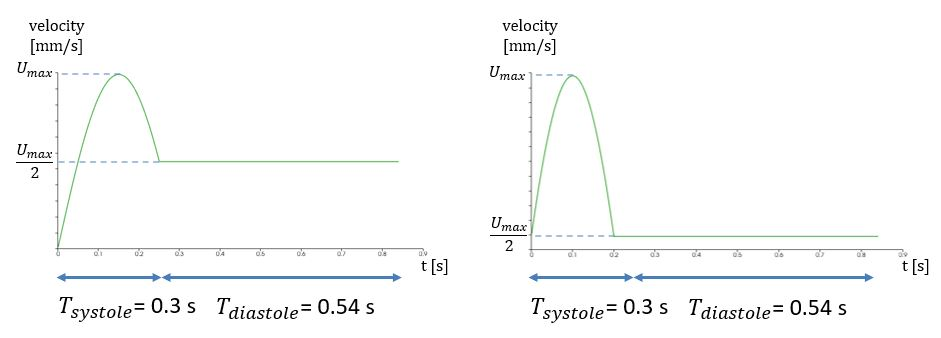
\includegraphics[width=\textwidth]{chapters/chp1/graphics/beat.JPG}
    %\caption{Left: time-dependency of the imposed inlet velocity profile in the preliminary simulation. Right: time-dependency of the imposed inlet velocity profile throughout a single heartbeat 0.8 s. The systolic and diastolic phase last 0.3 s and 0.54 s, respectively.}
   % \label{fig:heartbeat}
%\end{figure}

%\subsubsection*{3DVar benchmark}
%\label{sec:3DSteadyId}


%\subsubsection*{AAA benchmark}
%\label{sec:3DSteadyReal}



%\subsubsection*{Patient-specific AAA Geometry in Transient Conditions}
%\label{sec:3DtransReal}
%The same AAA geometry was used to evaluate transient inlet velocity profiles and observations across all 4DFlow acquisition time frames. 
%This test aimed to assess method stability under high Reynolds number conditions within a complex geometry. 
%Additional metrics included Time Averaged WSS (TAWSS) and Oscillatory Shear Index (OSI).

\section*{Results}
\label{sec:Results}
\label{ch:chapter_three}

\subsection*{Computational costs}
Numerical experiments were conducted on various setups: a workstation with 24 CPUs and 64 GB RAM for 2DVar and 3DVar and a high-performance computing system with 40 CPUs and 190 GB RAM for 2DVar+t and AAA benchmark. 2DVar took 30 minutes and 3DVar took 6 hours on 12 CPUs; on the other side, 6 hours were required for 2DVar+t and 17 hours for AAA benchmark.

%\subsection*{Benchmark Tests}
%\subsubsection*{2D Straight Conduit in Steady-State Conditions}
%Once the Tape was obtained, the value of \(RMSE\) between the computed and observed velocity fields was and 142.6 mm/s. The sensitivity of the VarDA approach to the spatial regularization parameter \(\alpha\) was tested with values from \(10^{-3}\) to \(10^{3}\). The lowest \(J + R\) was achieved at \(\alpha = 10^{-3}\), but did not correspond to the lowest \(RMSE\). Increasing \(\alpha\) to \(10^{0}\) resulted in the lowest \(RMSE\) and eliminated the velocity peak at the inlet. Higher values of \(\alpha\) (\(10^{2}\) and \(10^{3}\)) led to poorer reconstructions, as reflected in higher \(J + R\) values and flatter velocity profiles, resulting in greater deviations from observed values.
\subsection*{Preliminary tests}
%In the development of the VarDA approach, the integration of the entire pipeline and computational efficiency were prioritized, with a focus on the IPCS splitting scheme. Preliminary tests compared IPCS and a Coupled scheme under steady-state conditions on idealized 2D geometries, both at high and low Reynolds numbers.
In high Reynolds tests, IPCS optimization reduced RMSE from 142.60 mm/s to 6.70 mm/s, while the coupled scheme faced convergence issues. In low Reynolds conditions, IPCS proved to be five times faster than the coupled scheme and achieved a final RMSE of 1.76 mm/s compared to 4.22 mm/s for the coupled scheme.
%Therefore, IPCS was preferred for subsequent tests due to its effectiveness and lower computational time compared to the Coupled scheme, which exhibited convergence problems.

\subsection*{Progressively Demanding Tests}
%Upon completing the Tape, the value of \(RMSE\) was 134.7 mm/s. 
%The sensitivity of the VarDA approach to the spatial (\(\alpha\)) and temporal (\(\beta\)) regularization parameters was tested. 
\textbf{\textit{2DVar + t benchmark}} - When a zero-velocity field was imposed as IC, the post-optimization velocity field showed inconsistencies with respect to the observations.
In particular, a high-velocity region just downstream of the inlet section was obtained, while low velocity values were computed in the rest of the domain.
%, as if the flow field was not fully developed due to the inertial effects associated to triggering the motion of an initially still fluid.
Moreover, these tests did not yield improvements by changing \(\alpha\), and increasing \(\beta\) further worsened the performance (Fig. \ref{fig:3.3}). 

\begin{figure}
    \centering
    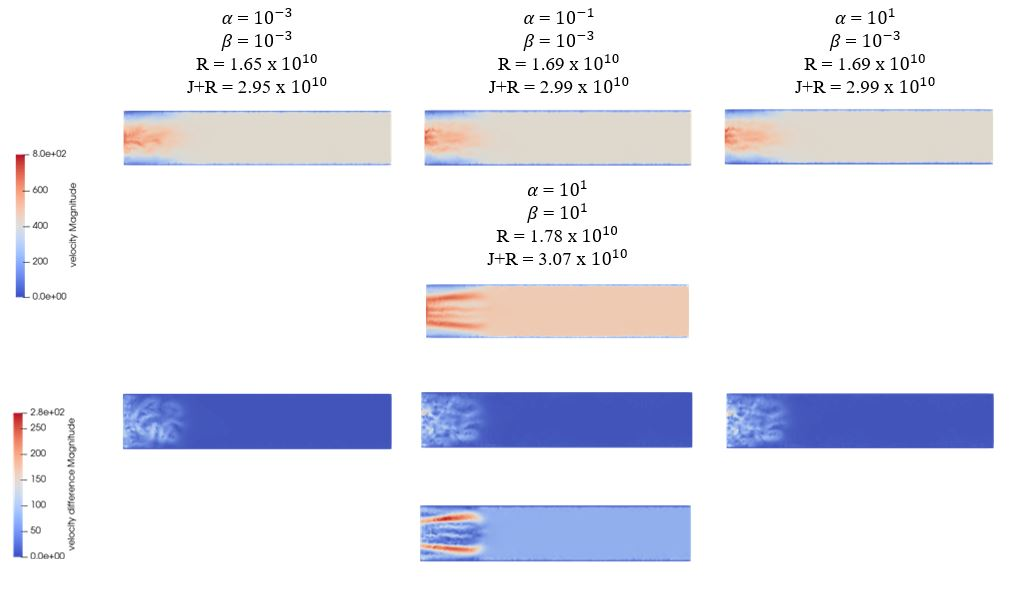
\includegraphics[width=0.65\textwidth, height = 0.25\textheight]{chapters/chp1/graphics/01.07_pt2.JPG}
    \caption{Sensitivity analysis of regularization parameters at systolic peak. First row: 2DVar + t velocity magnitude for different $\alpha$ values ($10^{-3}$, $10^{-1}$, $10^{1}$), with $\beta = 10^{-3}$. Second row: test with $\beta = 10^{1}$ to assess time regularization. Third and fourth rows: velocity difference between reference and 3DVar results for each $\alpha$ and $\beta$.}
    \label{fig:3.3}
\end{figure}

When the initial velocity and pressure fields were set equal to those yielded by the previous post-optimization simulation, the results showed a more homogeneous flow better matching parabolic characteristics and with lower \(J + R\) values.\\

%\subsection*{3DVar benchmark}
%After obtaining the Tape, the value of \(RMSE\) was 100.4 mm/s. 
\textbf{\textit{3DVar benchmark}} - VarDA was performed with spatial regularization terms set to $\alpha = 10^{-2}$, $10^1$, and $10^3$. The lowest value of $J + R$ was achieved with $\alpha = 10^{-2}$, but it did not correspond to the lowest RMSE. The velocity field exhibited a peak near the inlet, suggesting continuity loss. For $\alpha = 10^1$, the lowest RMSE was achieved, and the post-optimization velocity field more accurately reflected the observed data. Increasing $\alpha$ to $10^3$ resulted in significant deviations from the observations, with unexpected velocity behaviors and higher values of $J + R$ and RMSE. This suggests that lower $\alpha$ values improve RMSE, while higher $\alpha$ values lead to smoother solutions, but can introduce inaccuracies when too large.\\

%\subsection*{AAA benchmark}
\textbf{\textit{AAA benchmark}} - In first tests, \(RMSE\) improved from 59.3 mm/s to 55.1 mm/s, indicating a better alignment with observations (Fig. \ref{fig:3.7a}). 
\begin{figure}
    \centering
    \begin{minipage}{\textwidth}
        \centering
        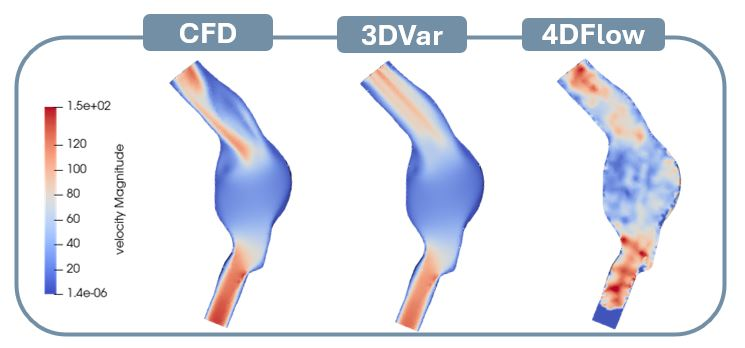
\includegraphics[width=0.47\textwidth, height = 0.15\textheight]{chapters/chp1/graphics/RealData3DVar.JPG}
        \subcaption{\small AAA benchmark velocity magnitude maps.}
        \label{fig:3.7a}
    \end{minipage}
    \\[1em]  % aggiungi spazio tra le immagini
    \begin{minipage}{\textwidth}
        \centering
        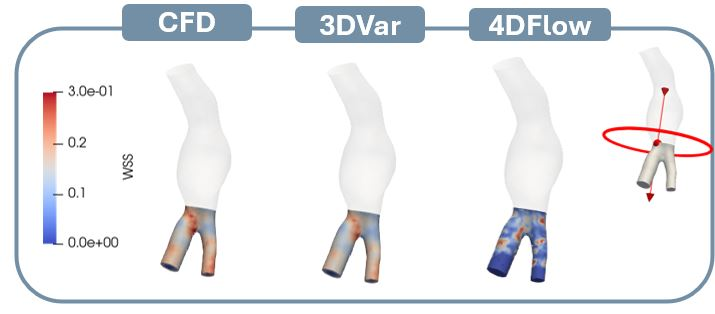
\includegraphics[width=0.47\textwidth, height = 0.15\textheight]{chapters/chp1/graphics/WSS3DVar.JPG}
        \subcaption{\small AAA benchmark WSS maps.}
        \label{fig:3.7b}
    \end{minipage}
    \caption{\small (a) velocity and (b) wall shear stress (WSS) fields obtained on the abdominal aortic aneurysm (AAA) computed by computational fluid dynamics (CFD) (\textbf{left}), derived directly from 4DFlow MRI (\textbf{right}), and by  data assimilation (\textbf{centre}).}
    \label{fig:3.7}
\end{figure}
Generating a Tape took about 25 minutes, while optimization required 17 hours with 80 Gb of memory. WSS distributions from Tape's output and 3DVar predictions were consistent, identifying regions with high shear stress (Fig. \ref{fig:3.7b}). WSS distributions from Tape's output and 3DVar predictions were consistent in terms of location of high WSS regions. Moreover, while enforcing consistency with 4DFlow-based velocity measurements, the 3DVar method yielded a regular and realistic WSS distribution. This is a major difference as compared to the WSS distribution estimated directly from 4DFlow data, which was unrealistic owing to their poor space-resolution and to the impact of noise in the near-wall region.


In tests with noisy observations, 3DVar effectively reconstructed the velocity field, slightly reducing \(RMSE\) from 36.8 mm/s to 36.4 mm/s, while maintaining WSS predictions consistent with CFD results, particularly at the iliac bifurcation, which is where the abdominal aorta splits into two smaller arteries, carrying blood to pelvis and legs.




\section*{Discussion}

%\subsection*{From 2D to 3D}
%2DVar and 3Dvar display distinct behaviors in sensitivity to regularization parameters. In 2DVar, the velocity field is poorly developed, especially when initialized with zero velocity, and varying $\alpha$ has minimal effect on optimization. Conversely, in 3DVar, moderate $\alpha$ values ($10^{1}$) significantly improve the velocity field, reducing inlet peaks and lowering \(RMSE\). However, excessive regularization ($\alpha = 10^{3}$) in 3DVar causes unrealistic velocity patterns.
%showing that the method is more sensitive in 3D conditions.

\subsection*{From 2DVar+t to 3DVar}
The 2DVar+t reveals challenges due to inertial effects and short simulation durations, causing reconstruction defects from incomplete flow development. Extending simulation time for optimization is impractical due to high computational costs. A potential solution includes proper initialization of CFD simulations and implementing a checkpointing method to reduce computational costs by using only the last cardiac cycle for gradient calculations.
Moreover, a key difference between 2DVar+t and 3DVar is the flow field's response to regularization. In 2DVar+t, increasing $\alpha$ has minimal effect due to dominant time-dependent effects, reducing spatial regularization's impact. Additionally, increasing $\beta$ deteriorates the results, a challenge not present in 3DVar, emphasizing the difficulty of balancing temporal and spatial regularization in dynamic flows. Conversely, in 3DVar, moderate $\alpha$ values ($10^{1}$) significantly improve the velocity field, reducing inlet peaks and lowering \(RMSE\). However, excessive regularization ($\alpha = 10^{3}$) causes unrealistic velocity patterns. 

%\subsection*{From 2D to 3D}
%The 2D steady-state tests emphasized the importance of the spatial regularization parameter $\alpha$ for velocity reconstruction quality. An optimal $\alpha = 10^{0}$ improved RMSE from 142.6 to 6.7, while higher values worsened the reconstruction. In 3D tests, $\alpha = 10^{1}$ was optimal, reducing RMSE from 100.4 to 15.2. However, further increases in $\alpha$ significantly degraded quality, highlighting the complexities of 3D simulations. The study underscores the critical role of spatial regularization  in boundary condition optimization problems in hemodynamics, with 3D tests requiring up to 80 GB of memory.


%\subsection*{From Steady-State to Transient}
%The 2DVar + time tests revealed challenges due to inertial effects and short simulation durations, causing reconstruction defects from incomplete flow development. Extending simulation time for optimization is impractical due to high computational costs. Varying $\alpha$ had minimal impact on reconstruction quality, and increasing $\beta$ did not yield significant improvements. A potential solution includes proper initialization of CFD simulations and implementing a checkpointing method to reduce computational costs by using only the last cardiac cycle for gradient calculations.

\subsection*{AAA benchmark}
AAA benchmark effectively reconstructs the velocity field in AAA geometry, maintaining high consistency with data obtained from 4D flow
imaging. It identifies high shear stress regions despite challenges due to lower resolution of 4D flow data near boundaries .
The method remains robust against noise. 

\section*{Conclusions}
This study demonstrates the application of the VarDA method to estimate optimal inlet BC for CFD simulations using noisy 4D flow MRI data. The method minimizes mismatch between CFD solutions and in vivo velocity data, producing a resolved, noise-free velocity field aligned with experimental measurements. Benchmarked on 2D and 3D geometries and applied to a patient-specific AAA geometry, it shows potential for personalized hemodynamic simulations. The IPCS framework improves efficiency and accuracy in transient flow analyses. Despite challenges in transient simulations, the work paves the way for future VarDA advancements, with implications for cardiovascular medicine.
%This study successfully demonstrates the application of the VarDA method to estimate an optimal inlet BC for CFD simulations, using noisy and uncertain 4D flow MRI data as input. The method effectively minimizes the mismatch between CFD solutions and in vivo velocity data, yielding a highly resolved and noise-free velocity field that aligns with experimental measurements. The method was benchmarked on ideal 2D and 3D geometries, and further applied to a patient-specific AAA geometry, highlighting its potential for personalized hemodynamic simulations. Additionally, the study showcases the computational advantages of the IPCS framework in improving efficiency and accuracy during transient flow analyses. Although challenges remain in transient flow simulations, this work paves the way for future enhancements in VarDA applications, with significant implications for cardiovascular medicine, particularly in surgical planning and device design.

%This project advances cardiovascular hemodynamic analysis by validating the VarDA method, demonstrating IPCS's superiority in computational efficiency and accuracy. While challenges in transient flow analyses remain, ongoing research will further enhance VarDA's application in cardiovascular medicine.

%\begin{acknowledgement}
%  I would like to express my gratitude to the \textit{Artery Project - Autonomous Robotics} for funding my participation in the FEniCS Conference and providing me with the opportunity to present my master's thesis project.
%  I would also like to express my heartfelt appreciation to Link\"oping University for supplying the 4D-Flow experimental data, which was essential for conducting the validation process.
%\end{acknowledgement}

\bibliographystyle{spbasic}
% Write the full path of your bibfile relative to book.tex
\bibliography{chapters/chp1/bibliography.bib}





\backmatter%%%%%%%%%%%%%%%%%%%%%%%%%%%%%%%%%%%%%%%%%%%%%%%%%%%%%%%
\appendix
%%%%%%%%%%%%%%%%%%%%%% appendix.tex %%%%%%%%%%%%%%%%%%%%%%%%%%%%%%%%%
%
% sample appendix
%
% Use this file as a template for your own input.
%
%%%%%%%%%%%%%%%%%%%%%%%% Springer-Verlag %%%%%%%%%%%%%%%%%%%%%%%%%%

\chapter{Chapter Heading}
\label{introA} % Always give a unique label
% use \chaptermark{}
% to alter or adjust the chapter heading in the running head

Use the template \emph{appendix.tex} together with the document class SVMono (monograph-type books) or SVMult (edited books) to style appendix of your book.


\section{Section Heading}
\label{sec:A1}
% Always give a unique label
% and use \ref{<label>} for cross-references
% and \cite{<label>} for bibliographic references
% use \sectionmark{}
% to alter or adjust the section heading in the running head
Instead of simply listing headings of different levels we recommend to let every heading be followed by at least a short passage of text. Further on please use the \LaTeX\ automatism for all your cross-references and citations.


\subsection{Subsection Heading}
\label{sec:A2}
Instead of simply listing headings of different levels we recommend to let every heading be followed by at least a short passage of text. Further on please use the \LaTeX\ automatism for all your cross-references and citations as has already been described in Sect.~\ref{sec:A1}.

For multiline equations we recommend to use the \verb|eqnarray| environment.
\begin{eqnarray}
\vec{a}\times\vec{b}=\vec{c} \nonumber\\
\vec{a}\times\vec{b}=\vec{c}
\label{eq:A01}
\end{eqnarray}

\subsubsection{Subsubsection Heading}
Instead of simply listing headings of different levels we recommend to let every heading be followed by at least a short passage of text. Further on please use the \LaTeX\ automatism for all your cross-references and citations as has already been described in Sect.~\ref{sec:A2}.

Please note that the first line of text that follows a heading is not indented, whereas the first lines of all subsequent paragraphs are.

% For figures use
%
\begin{figure}[t]
\sidecaption[t]
% Use the relevant command for your figure-insertion program
% to insert the figure file.
% For example, with the graphicx style use
\includegraphics[scale=.65]{figure}
%
% If no graphics program available, insert a blank space i.e. use
%\picplace{5cm}{2cm} % Give the correct figure height and width in cm
%
\caption{Please write your figure caption here}
\label{fig:A1}       % Give a unique label
\end{figure}

% For tables use
%
\begin{table}
\caption{Please write your table caption here}
\label{tab:A1}       % Give a unique label
%
% Follow this input for your own table layout
%
\begin{tabular}{p{2cm}p{2.4cm}p{2cm}p{4.9cm}}
\hline\noalign{\smallskip}
Classes & Subclass & Length & Action Mechanism  \\
\noalign{\smallskip}\hline\noalign{\smallskip}
Translation & mRNA$^a$  & 22 (19--25) & Translation repression, mRNA cleavage\\
Translation & mRNA cleavage & 21 & mRNA cleavage\\
Translation & mRNA  & 21--22 & mRNA cleavage\\
Translation & mRNA  & 24--26 & Histone and DNA Modification\\
\noalign{\smallskip}\hline\noalign{\smallskip}
\end{tabular}
$^a$ Table foot note (with superscript)
\end{table}
%

%%%%%%%%%%%%%%%%%%%%%%acronym.tex%%%%%%%%%%%%%%%%%%%%%%%%%%%%%%%%%%%%%%%%%
% sample list of acronyms
%
% Use this file as a template for your own input.
%
%%%%%%%%%%%%%%%%%%%%%%%% Springer Nature%%%%%%%%%%%%%%%%%%%%%%%%%%

\Extrachap{Glossary}


Use the template \emph{glossary.tex} together with the Springer Nature document class SVMono (monograph-type books) or SVMult (edited books) to style your glossary\index{glossary} in the Springer Nature layout.


\runinhead{glossary term} Write here the description of the glossary term. Write here the description of the glossary term. Write here the description of the glossary term.

\runinhead{glossary term} Write here the description of the glossary term. Write here the description of the glossary term. Write here the description of the glossary term.

\runinhead{glossary term} Write here the description of the glossary term. Write here the description of the glossary term. Write here the description of the glossary term.

\runinhead{glossary term} Write here the description of the glossary term. Write here the description of the glossary term. Write here the description of the glossary term.

\runinhead{glossary term} Write here the description of the glossary term. Write here the description of the glossary term. Write here the description of the glossary term.
\printindex

%%%%%%%%%%%%%%%%%%%%%%%%%%%%%%%%%%%%%%%%%%%%%%%%%%%%%%%%%%%%%%%%%%%%%%

\end{document}

